\graphicspath{{Chapters/ObjEventSelection/Figures/}}
\chapter{Object and Event Selection}
\label{chap:ObjEventSelection}

\section{Electron Selection}
\label{sec:objsel-el}

Electron reconstruction and identification was described in~\sec{reco-el}. Both
central electrons with \modetalt{2.47} and forward electrons are used. In
addition to the indentification requirements described in~\sec{reco-el}
additional selection requirements are imposed to select electrons likely to have
originated from \Z\ boson decays and to reject backgrounds. The requirements are
slightly different for the 8 \tev\ analysis compared to the 7 \tev\ analysis,
reflecting the different experimental conditions (such as higher pile-up in
2012) as well as optimisations made in 2012. The electron selection requirements
are summarised in~\tab{objsel-el} are described in more detail below. 

\begin{table}[]
  \centering
%   \vspace*{-1cm}
%\small
  \begin{tabular}{ l  l l }
    \hline\hline 
      Requirement        & 7 \tev\ & 8 \tev\ \\ 
      \hline
      \bf{Central Electron Selection} & \\
      Algorthim             & Standard (with GSF refit)     & Standard \\
      Quality               & Good Data Quality & \it{Same} \\
      ID cut                & \loosePP & \it{Same}       \\
      $\eta$                & $|\eta|<2.47$ & \it{Same} \\
      $E_T$                 & $E_T > 7$ GeV & \it{Same} \\
      $z_0$                 & $z_0 < 2$ mm & \it{Same} \\
      $d_0$                 & $|d_0|/\sigma(d_0) < 6 $ & \it{Same} \\
      Track isolation       & \ptconetwentylt{0.15} & \it{Same}   \\
      Calorimeter isolation & \etconetwentylt{0.3}          & \it{Not Applied} \\
      Overlap removal       & \multicolumn{1}{p{6cm}}{a) Remove $e$ if $\Delta R < 0.1$ from $\mu$} & \it{Same} \\
                            & \multicolumn{1}{p{6cm}}{b) Remove lowest $E_T$ $e$ in \deltaRlt{0.1} from another $e$} & \it{Same} \\ 
      \hline
      \bf{Forward Electron Selection:} & \\
      Alogirthm             & Forward & \it{Same} \\
      Quality               & Good Data Quality & \it{Same}  \\
      ID cut                & Tight & \it{Same} \\
      $\eta$                & $2.50<|\eta|<3.16$ & \it{Same} \\
      $E_T$                 & $E_T > 20$ GeV & \it{Same} \\
      Overlap removal       & \multicolumn{1}{p{6cm}}{Remove if overlaps with central electron or any muon in \deltaRlt{0.1}} & \it{Same}\\
%
      %\bf{Central Electron Selection} & \\
      %Algorthim             & Standard (with GSF refit)     & Standard \\
      %Quality               & \multicolumn{2}{c}{\texttt{(OQ  AND 1446 == 0})} \\
      %ID cut                & \multicolumn{2}{c}{\loosePP}       \\
      %$\eta$                & \multicolumn{2}{c}{$|\eta|<2.47$} \\
      %$E_T$                 & \multicolumn{2}{c}{$E_T > 7$ GeV} \\
      %$z_0$                 & \multicolumn{2}{c}{$z_0 < 2$ mm} \\
      %$d_0$                 & \multicolumn{2}{c}{$|d_0|/\sigma(d_0) < 6 $} \\
      %Track isolation       & \multicolumn{2}{c}{\ptconetwentylt{0.15}}   \\
      %Calorimeter isolation & \etconetwentylt{0.3}          & \it{Not Applied} \\
      %Overlap removal       & \multicolumn{2}{c}{a) Remove $e$ if $\Delta R < 0.1$ from $\mu$} \\
      %                      & \multicolumn{2}{c}{b) Remove lowest $E_T$ $e$ in \deltaRlt{0.1} from another $e$} \\ 
      %\hline
      %\bf{Forward Electron Selection:} & \\
      %Alogirthm             & \multicolumn{2}{c}{Forward} \\
      %Quality               & \multicolumn{2}{c}{\texttt{(OQ  AND 1446 == 0)}}  \\
      %ID cut                & \multicolumn{2}{c}{Tight} \\
      %$\eta$                & \multicolumn{2}{c}{$2.50<|\eta|<3.16$} \\
      %$E_T$                 & \multicolumn{2}{c}{$E_T > 20$ GeV} \\
      %Overlap removal       & \multicolumn{2}{p{8cm}}{\centering Remove if overlaps with central electron or any muon in \deltaRlt{0.1}} \\
    \hline \hline
  \end{tabular}
   \caption{Electron selection requirements.}
   \label{table:objsel-el}
\end{table}

\subsection{Central Electron Selection}

`Central' electrons, with \modetaclusterlt{2.47}, are reconstructed using the
``standard'' electron algorithm as described in~\sec{reco-el-reco}.  For 2011
data, the algorithm used was slightly different to the `standard' ATLAS electron
econstruction as tracks were refitted using a Gaussian-sum filter (GSF) to
account to account for the effect of bremsstrahlung in the inner detector. In
2012 data this became the default reconstruction algorithm. Central electrons
are required to pass the \loosePP\ identification algorithm.
%Electrons in the calorimeter ``crack" region $1.37 < |\eta_{cluster}| < 1.52$
%are included, although the efficiency and energy resolution is expected

For electron candidates with 4 or more silicon (SCT and Pixel) hits, the energy
of the electron is taken from the cluster measurement, and the eta and phi are
taken from the track (this requirement is automatically satisfied if the
electrons pass the \loosePP\ identification requirements). For electron
candidates with fewer than 4 silicon hits, all electron parameters are taken
directly from the cluster. In both cases, the cluster $\eta$ and $\phi$ are used for
the $\eta$ requirement and for overlap removal. Using the energy and direction
defined in this way, the electron candidates are required to have \etgt{7},
where \et\ is defined as $E\sin(\theta)=E/\cosh(\eta)$. 

A small number of the front-end boards of the liquid argon calorimeter were
inactive in 2011 and 2012; the exact number varied with time as some were
repaired whilst other developed faults. Additional, a number of individual cells
are masked in the readout (i.e. have their energy set to zero) due to
consistently producing high noise or failing to give a readout. There are also
regions where the High-Voltage supply to the LAr is faulty. Electrons are
rejected if they fall into a region of
$\eta, \phi$ space consistent with the presence of a dead front-end board in
the first or second sampling layer, the presence of a dead HV region affecting the
three samplings, or the presence of a masked cell in the core of the cluster.

To ensure that the candidates come from the primary vertex (defined as the
vertex that has the highest $\sum{\pt^2}$ of associated tracks), the
longitudinal impact parameter \zzero\ of the electron track with respect to the
primary vertex must be less than 2 mm. The \intro{unbiased} impact paramter is
used; the unbiased impact parameter for a particular track is obtained by
refitting the vertex without the track in question, then calculating the impact
parameter with respect to this refitted vertex, thus removing the pull of the
track from the vertex fit.  The transverse impact parameter \dzero\ must have a
significance (\dzero\ divided by the error on its measurement, \dzerosig) less
than 6. This helps reduce backgrounds, particularly from decays of pions and
kaons in jets to electrons, since these decays will occur further from the
interaction point giving larger impact parameters.

Isolation requirements are imposed to reduce the backgrounds from jets being
misidentified as electrons, or from electrons from decays in jets, collectively
referred to as \intro{background electrons}. Such background electrons will
typically have many tracks surrounding their track in the tracker, and be
surrounded by large energy deposits in the calorimeter from other particles in
the jet. \intro{Track Isolation} requirements are imposed, requiring that the
sum of the \pt\ of tracks surrounding the electron's track in a cone of
\deltaRlt{0.2} be less than 15\% of the electron's \pt, i.e.
\ptconetwentylt{0.15}. Tracks included in the calculation are required to have
\ptgt{0.4}, have impact parameters consistent with the same vertex as the
electron and have at least 9 silicon hits, thus ensuring good track quality and
purity. The impact parameter requirement means that this variable is insensitive
to pileup as most tracks from other (pileup) vertices are excluded.
Additionally, for the 2011 data, a calorimeter isolation requirement is imposed.
This is defined as the sum of calorimeter cell energies in a cone of
deltaRlt{0.2} around the barycentre of the electron cluster, excluding a 5x7
grid of cells in the centre of the cone (which are assumed to be due to the
electron). Cells from both the EM and hadronic calorimeters are included. The
requirement is that the sum of such energies be less than 30\% of electron \et,
i.e. \etconetwentylt{0.3}.  This variable is particularly sensetive to pileup,
as pileup events tend to deposit additional energy isotropically throughout the
detector, thus increasing the energy in the isolation cone. A correction
paramaterised by the number of vertices reconstructed in the event is applied to
reduce the effects of pileup.  Additional corrections are applied to correct for
leakage of the electron's energy out of the core cells of the cone, which tends
to increase with \pt.

Electrons closer than \deltaRlt{0.1} to a muon which passes the object selection
requirements (see~\sec{objsel-mu}) are rejected. If two selected electrons
overlap within \deltaRlt{0.1}, the lower-\et\ electron is removed, although in
the case of a central electron overlapping with a forward electron, which could
occur near the edge of the tracker, the central electron would take precedence.

\subsection{Forward Electron Selection}

Electrons reconstructed using the forward electron reconstruction algorithm are
used to to extend the pesudo-rapidity coverage beyond the limit of the tracker,
\modetaeq{2.5}. Only elecrons falling in the EMEC region are used, with
pseudo-rapidity \modetaclusterbetween{2.5}{3.16}.  Since the lack of tracking makes it
harder to reject hadronic and photonic fakes, these electrons are required to
pass tighter identification requirements: ``Forward Tight''. Since these
electrons lack a track measurement, it is impossible to determine their charge,
and of course impossible to apply track isolation and track parameter cuts.
Forward electrons are required to have \etgt{20}; this higher energy requirement
is motivated by the difficulty of measuring reconstruction and identification
efficiencies in data below this energy and by the higher hadronic and photonic
backgrounds at low energy.
%For this reason a tighter calorimeter isolation requirement is applied: the sum
%of the calorimeter transverse energy in a cone of $\Delta R = 0.3$ around the
%electron, removing the electron energy, must be less than 10\% of the electron
%energy.

\begin{figure}[h]
\centering
	\subfigure[]{
            \includegraphics[width=0.47\textwidth]{ObjSel/h_4l_ElEtCone20_log}
        }
	\subfigure[]{
            \includegraphics[width=0.47\textwidth]{ObjSel/h_4l_ElPtCone20_log}
        }
	\subfigure[]{
            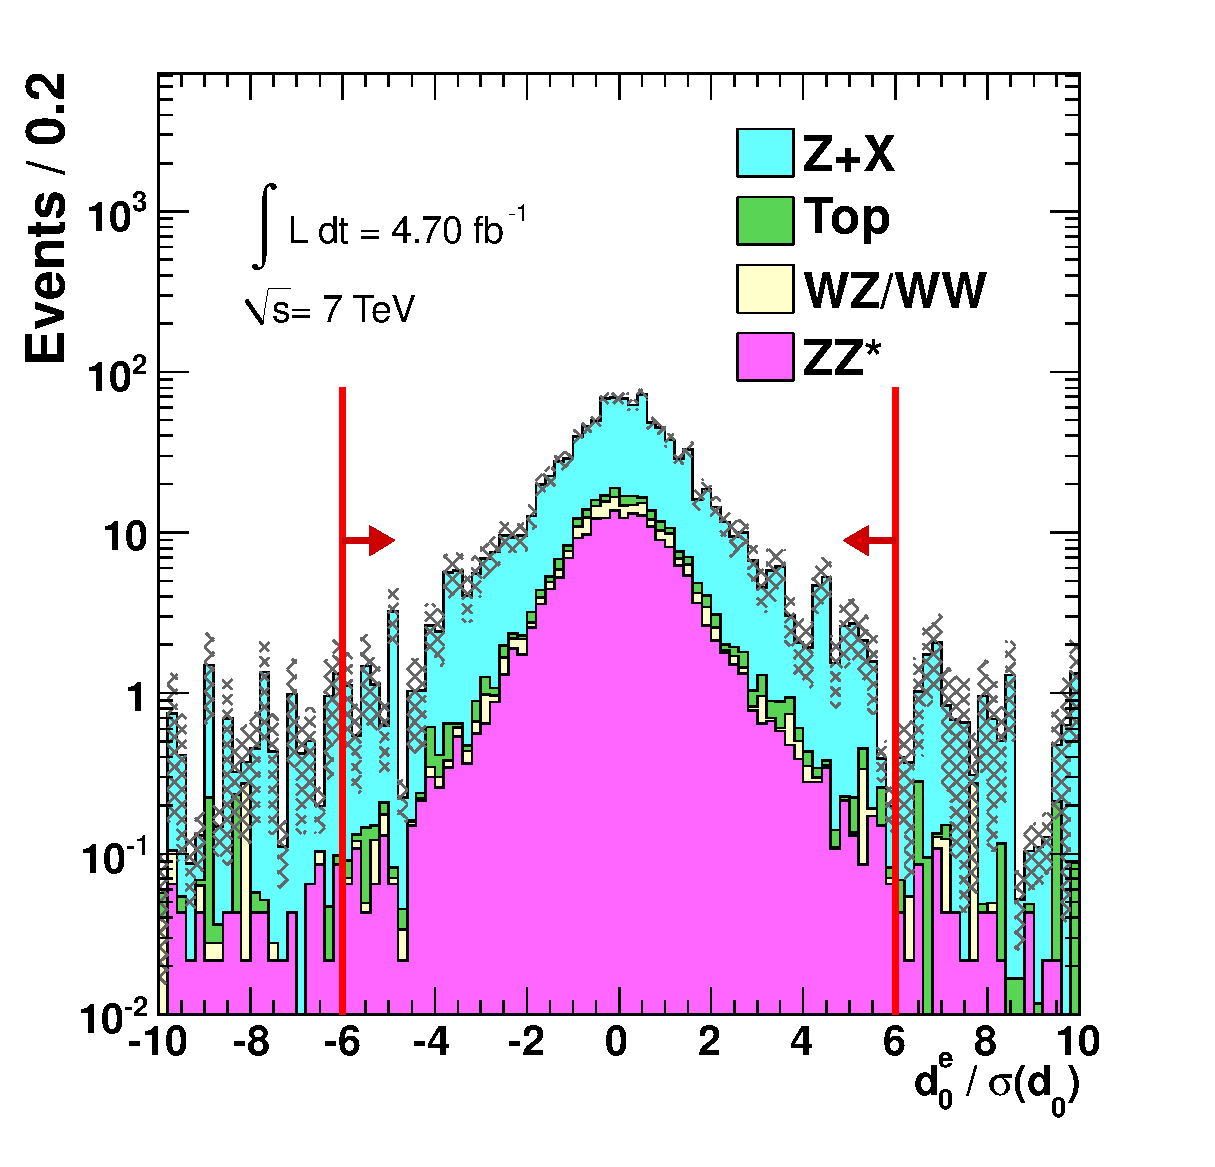
\includegraphics[width=0.47\textwidth]{ObjSel/h_4l_Electron_d0Sig_log}
        }
\caption[ ]{}
\label{fig:objsel-el}
\end{figure}

\section{Muon Selection}

\begin{table}[]
  \centering
%   \vspace*{-1cm}
\small
  \begin{tabular}{ l  l l }
    \hline\hline 
      Requirement        & 7 \tev\ & 8 \tev\ \\ 
      \hline
      \bf{Central Muons} & \\
      Algorithm             & \staco                        & \same \\
      Type                  & Combined or Segment Tagged    & \same \\
      $\eta$                & $|\eta|<2.5$                  & \same \\
      $p_T$                 & $p_T > 7$ GeV                 & \same \\
      ID Track Quality      & & \\
       - B Layer Hits       & $\geq 1$                         & \same \\
       - Pixel Hits         & $\geq 2$                         &  $\geq 1$\\
       - SCT Hits           & $\geq 6$                         &  $\geq 5$\\
       - Silicon `Holes'    & $<3$                          & \same \\
       - TRT                & \multicolumn{1}{p{5cm}}{\raggedright
                                {\bf If \modetalt{1.9}:} 
                                Require $n_{hits}+n_{outliers}>5$ 
                                and $n_{outliers}/(n_{hits}+n_{outliers})<0.9$}
                                                            & \multicolumn{1}{p{5cm}}{\raggedright
                                                                {\bf If \modetabetween{0.1}{1.9}:} 
                                                                Require $n_{hits}+n_{outliers}>5$ 
                                                                and $n_{outliers}/(n_{hits}+n_{outliers})<0.9$} \\
                            & \multicolumn{1}{p{5cm}}{\raggedright
                                {\bf If \modetagt{1.9}:} 
                                If $n_{hits}+n_{outliers}>5$ 
                                require $n_{outliers}/(n_{hits}+n_{outliers})<0.9$} 
                                                            & \multicolumn{1}{p{5cm}}{\raggedright
                                                                {\bf If \modetagt{1.9} or \modetalt{0.1}:} 
                                                                If $n_{hits}+n_{outliers}>5$ 
                                                                require $n_{outliers}/(n_{hits}+n_{outliers})<0.9$} \\
      $z_0$                 & $|z_0| < 2$ mm & $|z_0\sin(\theta)| < 0.5$ mm \\
      $d_0$                 & $|d_0|/\sigma(d_0) < 3.5 $ & \same \\
      Track isolation       & \ptconetwentylt{0.15} & \same   \\
      Calorimeter isolation & \etconetwentylt{0.3}          & \it{Not Applied} \\
      \hline
      \bf{Forward Muons} & \\
      Algorithm             & \staco                        & \same \\
      Type                  & Combined or Stand-Alone       & \same \\
      $\eta$                & \modetabetween{2.5}{2.7}      & \same \\
      $p_T$                 & $p_T > 10$ GeV                & \same \\
      % This is a cut that is automatically satisfied by combined
      %MS Track Quality      & Hits in all 3 stations        & \same \\
      ID Track Quality      & \multicolumn{2}{l}{\it Only apply to Combined Muons}  \\
       - B Layer Hits       & $\geq 1$                         & \same \\
       - Pixel Hits         & $\geq 2$                         &  $\geq 1$\\
       - SCT Hits           & $\geq 4$                         &  $\geq 3$\\
       - Silicon `Holes'    & $<3$                          & \same \\
      $z_0$                 & $|z_0| < 2$ mm & $|z_0\sin(\theta)| < 0.5$ mm \\
      $d_0$                 & $|d_0|/\sigma(d_0) < 3.5 $ & \same \\
      Calorimeter isolation & \etconetwentylt{0.15}          & \same \\

%
      %\bf{Central Electron Selection} & \\
      %Algorthim             & Standard (with GSF refit)     & Standard \\
      %Quality               & \multicolumn{2}{c}{\texttt{(OQ  AND 1446 == 0})} \\
      %ID cut                & \multicolumn{2}{c}{\loosePP}       \\
      %$\eta$                & \multicolumn{2}{c}{$|\eta|<2.47$} \\
      %$E_T$                 & \multicolumn{2}{c}{$E_T > 7$ GeV} \\
      %$z_0$                 & \multicolumn{2}{c}{$z_0 < 2$ mm} \\
      %$d_0$                 & \multicolumn{2}{c}{$|d_0|/\sigma(d_0) < 6 $} \\
      %Track isolation       & \multicolumn{2}{c}{\ptconetwentylt{0.15}}   \\
      %Calorimeter isolation & \etconetwentylt{0.3}          & \it{Not Applied} \\
      %Overlap removal       & \multicolumn{2}{c}{a) Remove $e$ if $\Delta R < 0.1$ from $\mu$} \\
      %                      & \multicolumn{2}{c}{b) Remove lowest $E_T$ $e$ in \deltaRlt{0.1} from another $e$} \\ 
      %\hline
      %\bf{Forward Electron Selection:} & \\
      %Alogirthm             & \multicolumn{2}{c}{Forward} \\
      %Quality               & \multicolumn{2}{c}{\texttt{(OQ  AND 1446 == 0)}}  \\
      %ID cut                & \multicolumn{2}{c}{Tight} \\
      %$\eta$                & \multicolumn{2}{c}{$2.50<|\eta|<3.16$} \\
      %$E_T$                 & \multicolumn{2}{c}{$E_T > 20$ GeV} \\
      %Overlap removal       & \multicolumn{2}{p{8cm}}{\centering Remove if overlaps with central electron or any muon in \deltaRlt{0.1}} \\
    \hline \hline
  \end{tabular}
   \caption{Electron selection requirements.}
   \label{table:objsel-el}
\end{table}

The reconstructed muons used in this analysis are reconstructed either using the
\verb|STACO| algorithm or the \verb|CaloTrkMuID| algoritm. 

In the \llll\ final state {\it Combined muons} (CM) and {\it Segment Tag muons}
(ST) are used in the pseudo-rapidity region $|\eta| < 2.5$, with $\pt>7$ GeV. 
Muons in the region $2.5 < |\eta| < 2.7$ are required to have a full muon spectrometer track,
which is combined with an inner-detector track if possible.
Only muons up to $|\eta|<2.6$ have such a chance, with decreasing probability 
as the $|\eta|$ increases; these Combined muons amount to $\sim 40\%$ of 
all muons with $2.5<|\eta|<2.6$ originating from \Z\ decays (see Figure 10 in reference \cite{ATL-COM-MUON-2011-026}). The rest of the muons in the $2.5<|\eta|<2.7$ region are Stand Alone muons, reconstructed using only the information from the muon system and are the only kind of muons reconstructed with $|\eta|>2.6$.
Muons with $|\eta| < 2.5$ are referred to as ``central muons'' and muons with
$2.5 < |\eta| < 2.7$ as ``forward muons''. 

\verb|CaloTrkMuID| muons use the calorimeter to tag inner-detector tracks as
originating from muons. This helps to recover efficieny at $|\eta|<0.1$ where
there is a gap in the muon-spectrometer. A muon with sufficient momentum
will traverse all the layers of the calorimeter, leaving a small signal. 
A low momentum hadron deposits
most of its energy in the first layers and leaves no signal in the last layers;
high momentum hadrons will deposit much energy in the core cells. 
Electrons will deposit much energy in the EM calorimeter. The \verb|CaloTrkMuID|
algorithm thus requires a MIP signal in each layer of the calorimeter to reject
hadron and electron backgrounds. A cut based quality selection and a likelihood
ratio based quality selection are both used, and we accept muons passing either.
\verb|CaloTrkMuID| muons are only used in the \llll\ final state for
$|\eta|<0.1$, and are not selected if they overlap with a selected \verb|STACO|
muon within $\Delta R<0.1$.

The muons must be isolated from energy deposits in the calorimeter. In the \llvv\
final-state, the
requirement is $etcone30/\pt < 0.15$. In the \llll\ final state the
requirement is $etcone20/\pt < 0.30$ for $|\eta|<2.5$ (all muon types) and
$etcone20/\pt < 0.15$ for $2.5<|\eta|<2.7$.
The energy in the cone is corrected for contributions from pile-up events using the number of vertices reconstructed in the event (\texttt{MuonIsolationCorrections-01-01}).

The inner detector track must be isolated from other tracks to reject secondary
muons from hadronic jets. In order to reject muons from the decay of heavy
quarks, in the \llvv\ final state we require the scalar sum of the transverse
momenta $(\Sigma \pt)$ of other tracks inside a cone of $\Delta R=0.3$ around
the muon to be no more than 15\% of the muon $\pt$. In other words, the
isolation requirement is $ptCone30/\pt < 0.15$. 

In both final states, inner detector tracks must have a minimum number of hits in each silicon sub-detector : at least 1 hit in the B-layer, $2$ in all Pixel layers, $6$ in the SCT, and less than 3 holes (no hit in a layer crossed by the track) in all silicon layers. For all those hit conditions, dead sensors count as hits observed, not as holes. Finally, a pseudo-rapidity dependent condition on TRT hits and outliers is applied, so that the TRT extension of the track is successful within the $\eta$ acceptance of the TRT (TRT hits can be associated as outliers when the extension is not successful)  : for $|\eta| < 1.9$, require 
$\mathrm{hits}+\mathrm{outliers} > 6$ and 
$\mathrm{outliers} < 0.9 \times (\mathrm{outliers}+\mathrm{hits})$; for $|\eta| > 1.9$, if $\mathrm{hits}+\mathrm{outliers} > 6$, require 
$\mathrm{outliers} < 0.9 \times (\mathrm{outliers}+\mathrm{hits})$~\cite{MCP}. 
  Forward muons must have hits on all three stations of the muon spectrometer
  track (inner, middle and outer). For forward tracks, a slightly looser set of quality cuts is applied to the number of hits in the silicon detectors: at least 1 hit in the B-layer, $2$ in all Pixel layers, $4$ in the SCT, and less than 3 holes (no hit in a layer crossed by the track) in all silicon layers. No cut is applied to the number of TRT hits.

To ensure that the candidates come from the primary vertex (identified as the
vertex that has the highest $\sum{\pt^2}$ of associated tracks), the magnitude
of the longitudinal impact parameter with respect to the primary vertex,
$|z_0|$, must be less than 2 mm and the transverse impact parameter, $d_0$, must
have significance ($|d_0|/\sigma_{d_0}$) less than 3.5. These requirements are not applied
to {\it Stand Alone muons} which have no inner-detector track.

\begin{figure}[h]
\centering
	\subfigure[]{
            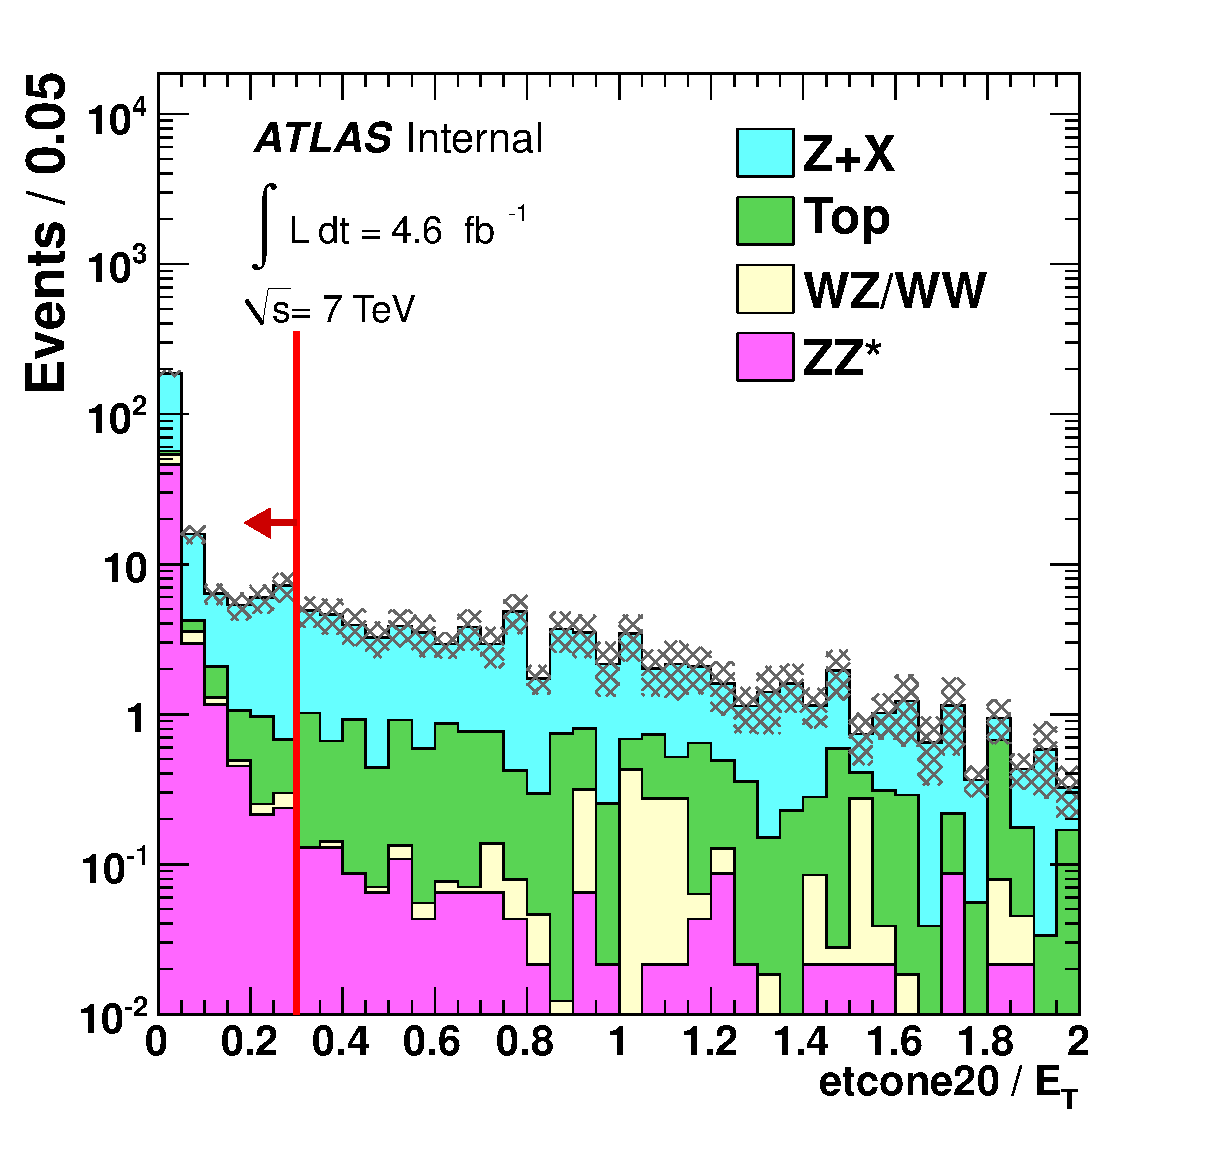
\includegraphics[width=0.47\textwidth]{ObjSel/h_4l_MuEtCone20_log}
        }
	\subfigure[]{
            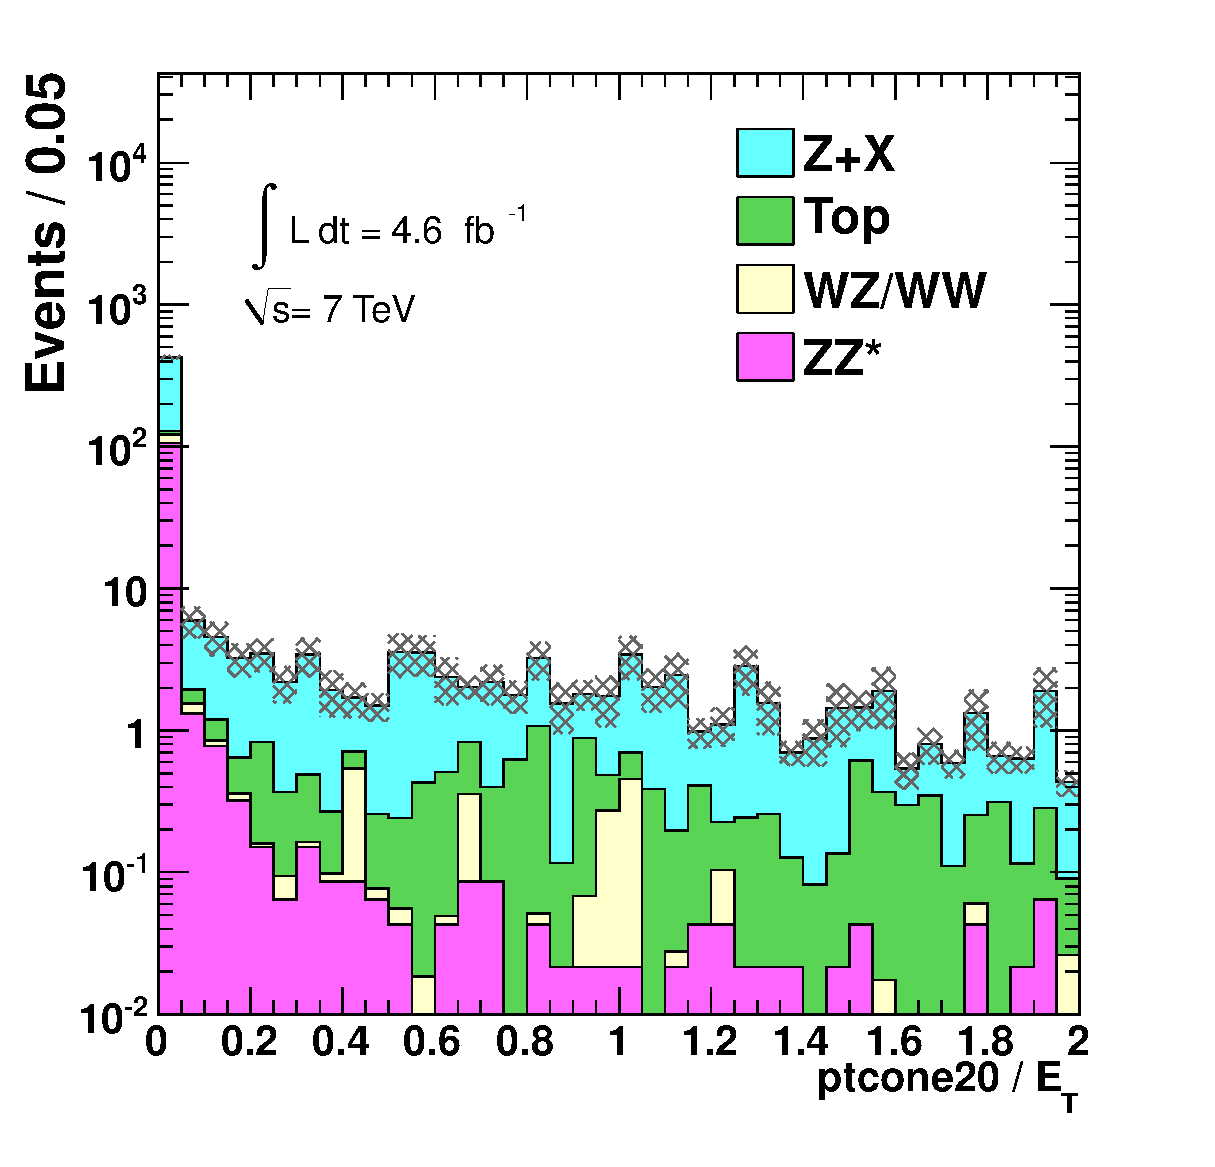
\includegraphics[width=0.47\textwidth]{ObjSel/h_4l_MuPtCone20_log}
        }
	\subfigure[]{
            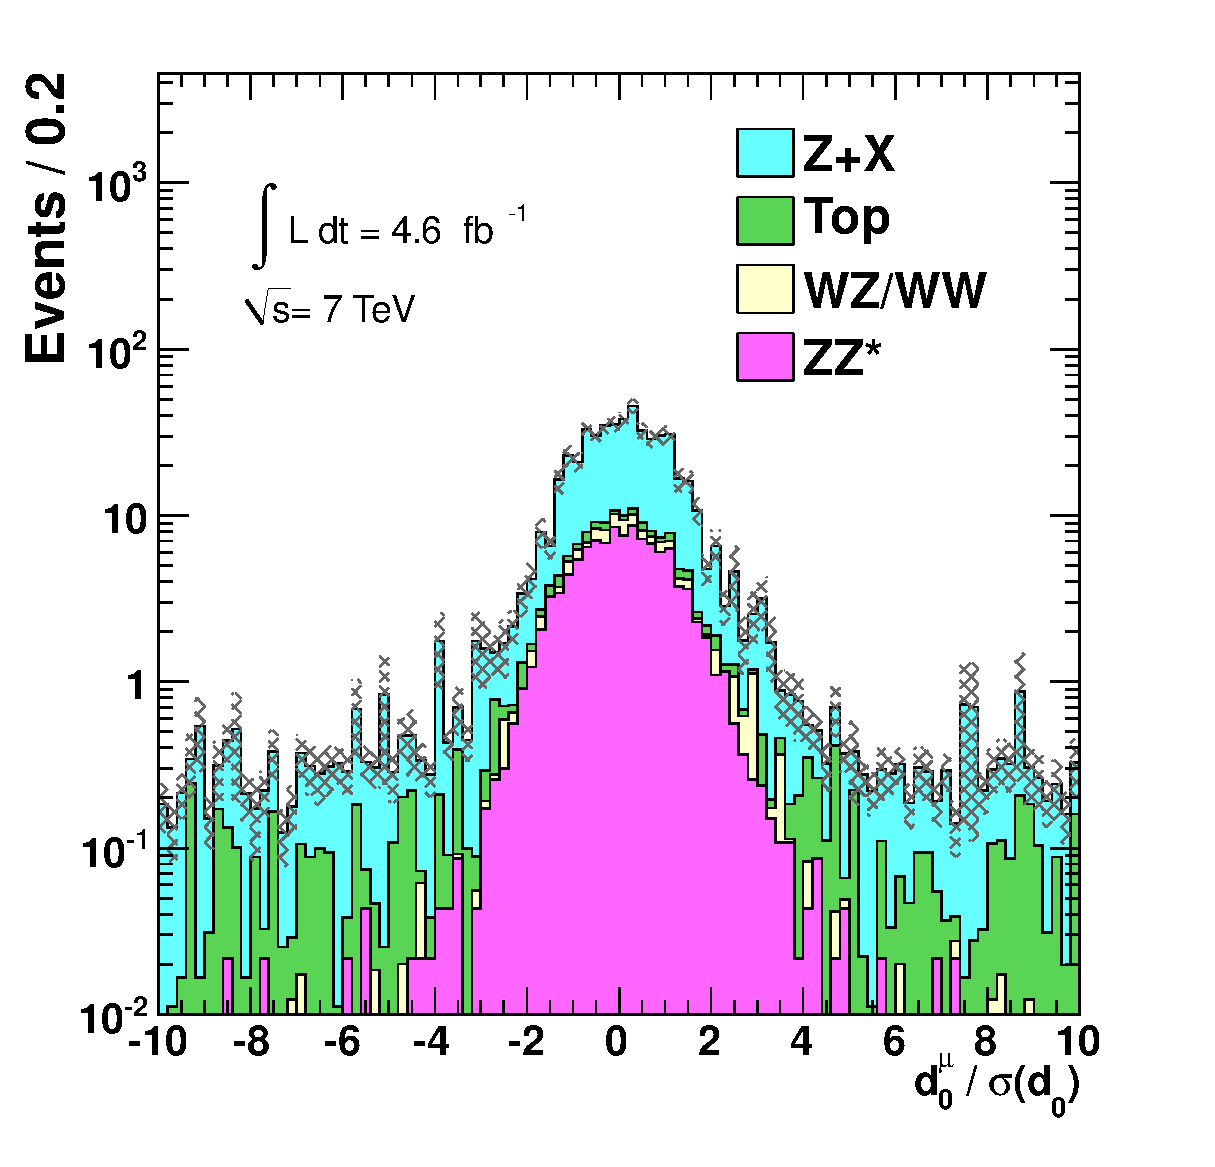
\includegraphics[width=0.47\textwidth]{ObjSel/h_4l_Muon_d0Sig_log}
        }
\caption[ ]{}
\label{fig:objsel-mu}
\end{figure}

\section{Jet Selection}
\section{\ZZ\ Event Selection}

Trigger MAtching and kin
\subsection{Triggers}
\section{Selection Efficiencies}
\subsection{\CZZ}
\subsection{Mispairing rates}
\subsection{Tau Contribution}
\section{Observed Kinematic Distributions}
